\def\chapname{Tracking of a Mobile Target}
\chapter[\chapname]
{\chapname \chapsubhead{The results of this chapter have been submitted in \cite{ammari2012tracking}}}

\label{chap:tracking}

\begin{abstract}
In this chapter we apply an extended Kalman filter to track both the
location and the orientation of a mobile target from the multistatic
response measurements described in chapter~\ref{chap:GPT-extraction}.
We also analyze the effect of the
limited-view aspect on the stability and the efficiency of our
tracking approach.
\end{abstract}



\section{Introduction}
\label{sec:intro}

% With each domain and material parameter, an infinite number of
% tensors, called the Generalized Polarization Tensors (GPTs), is
% associated. The concept of GPTs was introduced in
% \cite{ammarisima02, ammari2004reconstruction}. The GPTs contain significant information
% on the shape of the domain \cite{AGKLY11, AK_MMS_03,
% ammari_generalized_2012-1}. It occurs in several interesting
% contexts, in particular, in low-frequency scattering
% \cite{dassios, ammari2004reconstruction}, asymptotic models of dilute composites (see
% \cite{milton2002theory} and \cite{AKT_AA_05}), in invisibility cloaking in
% the quasi-static regime \cite{AKLL11} and in
% potential theory related to certain questions arising in
% hydrodynamics \cite{PS51}.
% 
% Another important use of this concept is for imaging diametrically
% small conductivity inclusions from boundary or multistatic
% response measurements. Multistatic response measurements are
% obtained using arrays of point source transmitters and receivers.
% This measurement configuration gives the so-called multistatic
% response matrix (MSR), which measures the change in potential
% field due to a conductivity inclusion. In fact, the GPTs are the
% basic building blocks for the asymptotic expansions of the
% perturbations of the MSR matrix due to the presence of small
% conductivity inclusions inside a conductor \cite{FV_ARMA_89,cedio1998identification,
% ammarisima02}. They can be reconstructed from the multi-static
% response (MSR) matrix by solving a linear system. The system has
% the remarkable property that low order generalized polarization
% tensors are not affected by the error caused by  the instability
% of higher orders in the presence of measurement noise. Based on
% the asymptotic expansion, efficient and direct (non-iterative)
% algorithms to determine the location and some geometric features
% of the inclusions were proposed. We refer to \cite{ammari2004reconstruction,
% ammari2007polarization} and the references therein for recent
% developments of this theory. An efficient numerical code for
% computing the GPTs is described in \cite{yves}.
% 
% 
% In \cite{ABGJKW2012dico}, we have analyzed the stability and
% the resolving order of GPT in a circular full angle of view
% setting with coincident sources and receivers, and developed
% efficient algorithms for target identification from a dictionary
% by matching the contracted GPTs (CGPTs). The CGPTs  are particular
% linear combinations of the GPTs (called harmonic combinations) and
% were first introduced in \cite{AKLL11}. As a
% consequence, explicit relations between the CGPT of scaled,
% rotated and translated objects have been established in
% \cite{ABGJKW2012dico}, which suggest strongly that the GPTs
% can also be used for tracking the location and the orientation of
% a mobile object. One should have in mind that, in real
% applications, one would like to localize the target and
% reconstruct its orientation directly from the MSR data without
% reconstructing the GPTs.


In this chapter we apply an extended Kalman filter to track both the
location and the orientation of a mobile target directly from MSR
measurements.

The Extended Kalman Filter (EKF) is a generalization of the Kalman
Filter (KF) to nonlinear  dynamical systems. It is robust with
respect to noise and computationally inexpensive, therefore is
well suited for real-time applications such as tracking
\cite{kalman2}.

Target tracking is an important task in sonar and radar imaging,
security technologies,  autonomous vehicle, and robotics. The
use of Kalman-type filtering for target tracking is quite
standard, see, for instance,
\cite{track1,track2,track3,track4,track5, track6}.

However, to the best of our knowledge, this is the first time
where tracking of the orientation of a target is provided.
Moreover, we analyze the ill-posed character of both the location
and orientation tracking in the case of limited-view data. In
practice, it is quite realistic to have the sources/receivers
cover only a limited angle of view. In this case, the
reconstruction of the GPTs becomes more ill-posed than in the
full-view case.


It is the aim of this chapter to provide a fast algorithm for
tracking both the location and the orientation of a mobile target, in the
toy model described in chapter~\ref{chap:GPT-extraction}.

The chapter is organized as follows. In
section \ref{sec:tracking_of_mobile_target} we present a GPT-based
location and orientation tracking algorithm using an extended
Kalman filter and show the numerical results in the full-view
setting. The chapter
ends with a few concluding remarks. A brief review of the extended
Kalman filter is given in appendix~\ref{sec:KalmanFilter}.

\newcommand{\bMD}{\bM_D}

\section{Tracking of a mobile target}
\label{sec:tracking_of_mobile_target}

In this section, we describe the setting of the tracking problem, and define
in detail the algorithm that will be used.

\subsection{Time dependent data acquisition}

Except for the few modifications below, we keep the notations that have been
used throughout chapters~\ref{chap:GPT-extraction}-\ref{chap:dico-matching}.


At the instant $t\geq 0$, we denote by $z_t=[x_t, y_t]^\top\in\R^2$ the location and
$\theta_t\in[0,2\pi)$ the orientation of a target $D_t$.
\begin{align}
  \label{eq:target_transrot_t}
  D_t=z_t+R_{\theta_t} D,
\end{align}
where $R_{\theta_t}$ is the rotation by $\theta_t$. Let $\bM_t$ be
the CGPT of $D_t$, and $\bMD$ be the CGPT of $D$. Then the
equation \eqref{eq:Vmodel} becomes
\begin{align}
  \label{eq:MSR_CGPT_linsys_time}
  \bV_t = L (\bM_t) + \mbf E_t + \bW_t,
\end{align}
where $\bE_t$ is the truncation error, and $\bW_t$ the measurement noise at time $t$.

The objective of \emph{tracking} is to estimate the target's location $z_t$ and
orientation $\theta_t$ from the MSR data stream $\bV_t$. We emphasize that these
informations are contained in the first two orders CGPTs as shown in 
chapter~\ref{chap:dico-matching}. Precisely, let $\Delta x_t=x_t-x_{t-1}$, $\Delta
y_t=y_t-y_{t-1}$ and $\Delta \theta_t=\theta_t-\theta_{t-1}$, then equations in
proposition~\ref{prop:complex-cgpt-under} become~:
\begin{equation}
  \label{eq:linsys_P1}
  \begin{aligned}
    % \frac{\No_{12}(D_t)}{\No_{11}(D_t)} &= 2(\Delta x_t + i\Delta y_t) + e^{i\Delta\theta_t} \frac{\No_{12}(D_{t-1})}{\No_{11}(D_{t-1})},\\
    % \nm
    % \frac{\Nt_{12}(D_t)}{\Nt_{11}(D_t)} &= 2(\Delta x_t + i\Delta y_t) + e^{i\Delta\theta_t} \frac{\Nt_{12}(D_{t-1})}{\Nt_{11}(D_{t-1})}.
    \No_{12}(D_t)/\No_{11}(D_t) &= 2(\Delta x_t + i\Delta y_t) + e^{i\Delta\theta_t} \No_{12}(D_{t-1})/\No_{11}(D_{t-1}),\\
    \nm
    \Nt_{12}(D_t)/\Nt_{11}(D_t) &= 2(\Delta x_t + i\Delta y_t) + e^{i\Delta\theta_t} \Nt_{12}(D_{t-1})/\Nt_{11}(D_{t-1}).
  \end{aligned}
\end{equation}
Hence when the linear system \eqref{eq:linsys_P1} is solvable, one
can estimate $z_t, \theta_t$ by solving and accumulating $\Delta
x_t, \Delta y_t$ and $\Delta \theta_t$. However, such an algorithm
will propagate the error over time, since the noise presented in
data is not properly taken into account here.

In the following we develop a CGPT-based tracking algorithm using the Extended Kalman
Filter, which handles correctly the noise. We recall first the definition of complex
CGPT, with which a simple relation between $\bM_t$ and $\bMD$ can be established.

\subsection{Time relationship between CGPTs}
Let $\oov=(1, i)^\top$. The complex CGPTs $\No, \Nt$ defined in
\eqref{eq:Mccdef} then verify~:
\begin{align*}
  N_{mn}^{(1)} &= (M_{mn}^{cc} - M_{mn}^{ss}) + i (M_{mn}^{cs} + M_{mn}^{sc}) = \oov^\top M_{mn} \oov, \\
  N_{mn}^{(2)} &= (M_{mn}^{cc} + M_{mn}^{ss}) + i (M_{mn}^{cs} - M_{mn}^{sc}) = \oov^H M_{mn}
  \oov,
\end{align*}
where $M_{mn}$ is the $2\times 2$ matrix defined by
$$
M_{mn} = \begin{pmatrix}
    M_{mn}^{cc} & M_{mn}^{cs} \\
    M_{mn}^{sc} & M_{mn}^{ss} \\
  \end{pmatrix},
$$
and $H$ denotes the Hermitian transpose. Therefore, we have
\begin{align}
  \label{eq:CCGPT_CGPT_mat}
  \No = \bU^\top \bM \bU  \quad \mbox{ and } \quad \Nt = \bU^H \bM \bU,
\end{align}
where the matrix $\bU$ of dimension $2K\times K$ over the complex
fields is defined by
\begin{align}
  \label{eq:def_U_mat}
  \bU =\begin{pmatrix}
    \oov & 0 & \ldots & 0\\
    0 & \oov & \ldots & 0\\
    \vdots & ~ & \ddots & \vdots \\
    0 & \ldots & 0 & \oov
  \end{pmatrix},
\end{align}
and $\bM$ is the matrix whose $(m,n)$ block is given by $M_{mn}$.

To recover the CGPT $\bM$ from the complex CGPTs $\No, \Nt$,
we simply use the relations
\begin{equation}
  \label{eq:CGPT_CCGPT_recovery}
  \begin{aligned}
    M_{mn}^{cc} &= \frac{1}{2} \Re(N_{mn}^{(1)} + N_{mn}^{(2)}), \ M_{mn}^{cs} = \frac{1}{2} \Im(N_{mn}^{(1)} + N_{mn}^{(2)}),\\
    M_{mn}^{sc} &= \frac{1}{2} \Im(N_{mn}^{(1)} - N_{mn}^{(2)}), \ M_{mn}^{ss} = \frac{1}{2} \Re(N_{mn}^{(2)} -
    N_{mn}^{(1)}),
  \end{aligned}
\end{equation}
where $\Re,\Im$ are the real and imaginary part of a complex
number, respectively. For two targets $D_t, D$ satisfying
\eqref{eq:target_transrot_t}, equations \eqref{eq:DB_tsr_No} and \eqref{eq:DB_tsr_Nt} give us
\begin{subequations}
  \label{eq:CCGPT_tsr}
  \begin{align}
    \No(D_t) &= \Fmat^\top \No(D) \Fmat, \\
    \Nt(D_t) &= \Fmat^H \Nt(D) \Fmat ,
    % \No(D_t) &= (\Ft) \No(D_0) (\Ft)^\top, \\
    % \Nt(D_t) &= (\overline\Ft) \Nt(D_0) (\Ft)
  \end{align}
\end{subequations}
where $\Fmat$ is a upper triangle matrix with the $(m,n)$-th entry given by
\begin{align}
  \label{eq:Fmat_mn}
  (\Fmat)_{mn} = \binom{n}{m} {(x_t + i y_t)}^{n-m}e^{im\theta_t} .
\end{align}
% $\mathbf{C}^z_{mn}= \binom{m}{n} z^{m-n}$, and $\bG^\theta$ is diagonal with
% the $m$-th diagonal element given by $e^{i\theta m}$.

\subsubsection*{Linear operator $\mbf T_t$:}
Now one can find explicitly a linear operator $\mbf T_t$ (the
underlying scalar field is $\R$) which depends only on $z_t,
\theta_t$, such that $\bM_t=\mbf T_t(\bMD)$, and the equation
\eqref{eq:MSR_CGPT_linsys_time} becomes
\begin{align}
  \label{eq:MSR_CGPT_linsys_time_Tt}
  \bV_t = L(\bT_t(\bMD)) + \bE_t + \bW_t .
\end{align}
For doing so, we set $\Jmat := \bU\Fmat$, where $\bU$ is given by
(\ref{eq:def_U_mat}). Then, a straightforward computation using
\eqref{eq:CCGPT_CGPT_mat}, \eqref{eq:CGPT_CCGPT_recovery}, and
\eqref{eq:CCGPT_tsr}  shows that
\begin{equation}
  \label{eq:CGPT_tsr}
  \begin{aligned}
    \Mcc(D_t) &= \Re \Jmat^\top \bMD \Re \Jmat, \ \Mcs(D_t) = \Re \Jmat^\top \bMD \Im \Jmat, \\
    \Msc(D_t) &= \Im \Jmat^\top \bMD \Re \Jmat, \ \Mss(D_t) = \Im \Jmat^\top \bMD \Im
    \Jmat,
    % \Mcc(D_t) &= \Re \Jmat^\top \bM(D_0) \Re \Jmat, \ \Mcs(D_t) = \Re \Jmat^\top \bM(D_0) \Im \Jmat, \\
    % \Msc(D_t) &= \Im \Jmat^\top \bM(D_0) \Re \Jmat, \ \Mss(D_t) = \Im \Jmat^\top \bM(D_0) \Im \Jmat
    % M_{mn}^{cc}(D) &= (\Re J^\top \bM(D_0) \Re J)_{mn}, \ M_{mn}^{cs}(D) = (\Re J^\top \bM(D_0) \Im J)_{mn}, \\
    % M_{mn}^{sc}(D) &= (\Im J^\top \bM(D_0) \Re J)_{mn}, \ M_{mn}^{ss}(D) = (\Im J^\top \bM(D_0) \Im J)_{mn}
  \end{aligned}
\end{equation}
where $\Mcc(D_t),\Mcs(D_t),\Msc(D_t),\Mss(D_t)$ are the matrices with 
coefficients $(m,n)$ defined in~\eqref{defc1}-\eqref{defc1}. Therefore, we get the
operator $\mbf T_t$:
\begin{align}
  \label{eq:def_op_Tt}
  \mbf T_t(\bMD) =\ &\Re \bU (\Re \Jmat^\top \bMD \Re \Jmat) \Re \bU^\top + \Re \bU (\Re \Jmat^\top
  \bMD \Im \Jmat) \Im \bU^\top + \notag \\
  &\Im \bU (\Im \Jmat^\top \bMD \Re \Jmat) \Re \bU^\top + \Im \bU (\Im \Jmat^\top \bMD \Im \Jmat) \Im
  \bU^\top = \bM_t .
\end{align}

\subsection{Tracking by the Extended Kalman Filter}
\label{sec:track-extend-kalm} The EKF is a generalization of the
KF to nonlinear dynamical systems. Unlike KF which is an optimal
estimator for linear systems with Gaussian noise, EKF is no longer
optimal, but it remains robust with respect to noise and
computationally inexpensive, therefore is well suited for
real-time applications such as tracking. We establish here the
\emph{system state} and the \emph{observation} equations which are
fundamental to EKF, and refer readers to Appendix
\ref{sec:extend-kalm-filt} for its algorithmic details.

\subsubsection{System state observation equations}
\label{sec:system_state_obsrv_eq}

We assume that the position of the target is subjected to an
external driving acceleration that has the form of a white noise.
In other words the velocity $({V}(\tau))_{\tau
  \in \R^+}$ of the target is given in terms of a two-dimensional Brownian motion
$({W}_a(\tau))_{\tau \in \R^+}$ and its position $({Z}(\tau))_{\tau \in \R^+}$ is
given in terms of the integral of this Brownian motion:
$$
{V}(\tau) = {V}_0 + \sigma_a  { W}_a(\tau), \quad \quad {Z}(\tau) = {Z}_0 + \int_0^\tau {V}(s) ds .
$$
The orientation  $(\Theta(\tau))_{\tau \in \R^+}$ of the target is subjected to random fluctuations and
its angular velocity is
given in terms of an independent white noise, so that the orientation
is  given in terms  of a one-dimensional Brownian motion $(W_\theta(\tau))_{\tau \in \R^+}$:
$$
\Theta(\tau) = \Theta_0+ \sigma_\theta W_\theta(\tau) .
$$
We observe the target at discrete times $t \Delta \tau$, $t \in \N$, with time step $\Delta \tau$.
We denote ${z}_t=  {Z}(t \Delta \tau)$, ${v}_t =  {V}(t \Delta \tau)$, and $\theta_t=  \Theta(t \Delta \tau)$.
They obey the recursive relations
\begin{equation} \label{eq:move_model}
  \begin{array}{ll}
\dis  {v}_t = {v}_{t-1}+ {a}_{t} ,
&\quad \dis {a}_{t}= \sigma_a  \big( {W}_a(t\Delta \tau) -{W}_a((t-1)\Delta \tau) \big), \\
\dis  {z}_t = {z}_{t-1}+ {v}_{t-1} \Delta \tau + {b}_{t} , &\quad
\dis {b}_{t}= \sigma_a  \int_{(t-1) \Delta \tau}^{t \Delta \tau}
{W}_a(s) -{W}_a((t-1)\Delta \tau)ds , \\
\dis  \theta_t = \theta_{t-1}+ c_{t} , &\quad \dis c_{t}=
\sigma_\theta  \big( W_\theta(t\Delta \tau) -W_\theta((t-1)\Delta
\tau) \big) .
\end{array}
\end{equation}
 Since the increments of the Brownian motions are independent from each other,
 the vectors $(U_t)_{t \geq 1}$ given by
 $$
 U_t=
 \begin{pmatrix}
 {a}_t\\
 {b}_t\\
 c_t\end{pmatrix}
 $$
 are independent and identically distributed
 with the multivariate normal distribution with mean zero and
 covariance matrix $\bSigma$ given by
 \begin{equation} \label{eq:noise_cov_matrix}
 \bSigma= \Delta \tau
 \begin{pmatrix}
 \sigma_a^2 {\bf I}_2 & \frac{\sigma_a^2}{2} \Delta \tau {\bf I}_2 &0\\
 \frac{\sigma_a^2}{2} \Delta \tau {\bf I}_2 & \frac{\sigma_a^2}{3} \Delta \tau^2 {\bf I}_2 & 0\\
 0 & 0 & \sigma_\theta^2
 \end{pmatrix}
 \end{equation}
 The evolution of the state vector
 $$
 X_t =
 \begin{pmatrix}
 {v}_t\\
 {z}_t\\
 \theta_t
 \end{pmatrix}
 $$
 takes the form
 \begin{equation} \label{eq:sys_state_matrix_form}
 X_t = \bF X_{t-1} + U_{t}, \quad \quad
 \bF=
 \begin{pmatrix}
 \bI_2 & 0 & 0\\
 \Delta \tau \bI_2 & \bI_2 & 0 \\
 0 & 0 & 1
 \end{pmatrix}
 \end{equation}




The observation made at time $t$ is the MSR matrix given by
\eqref{eq:MSR_CGPT_linsys_time_Tt}, where the system state $X_t$
is implicitly included in the operator $\bT_t$. We suppose that
the truncation error $\bE_t$ is small compared to the measurement
noise so that it can be dropped in
\eqref{eq:MSR_CGPT_linsys_time_Tt}, and that the Gaussian white
noise $\bW_t$ of different time are mutually independent. We
emphasize that the velocity vector $v_t$ of the target does not
contribute to \eqref{eq:MSR_CGPT_linsys_time_Tt}, which can be
seen from \eqref{eq:target_transrot_t}. To highlight the
dependence upon $z_t, \theta_t$, we introduce a function
$\mathbf{h}$ which is nonlinear in $z_t, \theta_t$, and takes
$\bMD$ as a parameter, such that
\begin{align}
  \label{eq:linsys_func_h}
  % h(z_t, \theta_t;\bMD) = L(\bT_t(\bMD)),
  \mathbf{h}(X_t; \bMD) = \mathbf{h}(z_t, \theta_t;\bMD) = L(\bT_t(\bMD)).
\end{align}
Then together with \eqref{eq:sys_state_matrix_form} we get the following \emph{system state} and
\emph{observation} equations:
\begin{subequations}
  \label{eq:sys_state_obs_eq}
  \begin{align}
      X_t &= \bF X_{t-1} + U_t , \label{eq:system_eq} \\
      \bV_t &= \mathbf{h}(X_t; \bMD) + \bW_t .\label{eq:observ_eq}
      % \bV_t &= L_t(\bT_t(\bMD)) + \bW_t \label{eq:observ_eq}
  \end{align}
\end{subequations}
Note that \eqref{eq:system_eq} is linear, so in order to apply EKF
on \eqref{eq:sys_state_obs_eq}, we only need to linearize
\eqref{eq:observ_eq}, or in other words, to calculate the partial
derivatives of $\mathbf{h}$ with respect to $x_t, y_t, \theta_t$.

\subsubsection{Linearization of the observation equation}
\label{sec:lin_obs_eq}

Clearly, the operator $L$ contains only the information
concerning the acquisition system and does not depend on $x_t,
y_t, \theta_t$. So by \eqref{eq:linsys_func_h}, we have
\begin{align}
  \label{eq:partial_h}
  \partial_{x_t}\mathbf{h}=L(\partial_{x_t}\bT_t(\bMD)),
%, \ \ \partial_{\theta_t}h=L_t(\partial_{\theta_t}\bT_t(\bMD)),
\end{align}
while the calculation for $\partial_{x_t}\bT_t$ is straightforward using
\eqref{eq:def_op_Tt}. We have %, see Appendix C for details.
\begin{align}
  \label{eq:derivatives_Tt}
  \partial_{x_t}\bT_t(\bMD) = &\Re \bU \partial_{x_t}(\Re \Jmat^\top \bMD \Re \Jmat) \Re \bU^\top +
  \Re \bU \partial_{x_t}(\Re \Jmat^\top \bMD \Im \Jmat) \Im \bU^\top + \notag \\
  &\Im \bU \partial_{x_t}(\Im \Jmat^\top \bMD \Re \Jmat) \Re \bU^\top + \Im \bU \partial_{x_t}(\Im
  \Jmat^\top \bMD \Im \Jmat) \Im \bU^\top ,
\end{align}
where the derivatives are found by the chain rule:
\begin{align*}
\partial_{x_t}(\Re \Jmat^\top \bMD \Re \Jmat) &= \Re (\partial_{x_t}\Jmat^\top) \bMD \Re
\Jmat+\Re\Jmat^\top \bMD \Re(\partial_{x_t}\Jmat),\\
\partial_{x_t}(\Re \Jmat^\top \bMD \Im \Jmat) &= \Re (\partial_{x_t}\Jmat^\top) \bMD
\Im \Jmat+\Re\Jmat^\top \bMD \Im(\partial_{x_t}\Jmat),\\
\partial_{x_t}(\Im \Jmat^\top \bMD \Re \Jmat) &= \Im (\partial_{x_t}\Jmat^\top)
\bMD \Re \Jmat+\Im\Jmat^\top \bMD \Re(\partial_{x_t}\Jmat),\\
\partial_{x_t}(\Im \Jmat^\top \bMD \Im \Jmat) &= \Im (\partial_{x_t}\Jmat^\top)
 \bMD \Im \Jmat+\Im\Jmat^\top \bMD \Im(\partial_{x_t}\Jmat),
\end{align*}
and $\partial_{x_t}\Jmat = \bU\partial_{x_t} \mathbf{F}_t$. The
$(m,n)$-th entry of the matrix $\partial_{x_t} \mathbf{F}_t$ is
given by
\begin{align}
  \label{derv_z_Ft}
  (\partial_{x_t} \mathbf{F}_t)_{m,n} = \binom{n}{m} (n-m) z_t^{n-m-1}
  e^{im\theta_t}.
\end{align}
The derivatives $ \partial_{y_t}\bT_t(\bMD)$ and $\partial_{\theta_t}\bT_t(\bMD)$ are calculated
in the same way.

\section{Numerical results}

In this section, we perform computation of such experiments of tracking.
We treat both the problem of full-view (subsection~\ref{sec:tracking_numexp_full_view})
and partial-view (subsection~\ref{sec:tracking_numexp_partial_view}) settings.

\subsection{Numerical experiments of tracking in the full-view setting}
\label{sec:tracking_numexp_full_view}

% In the first experiment we show the performance of EKF in a full angle of view setting with the
% letter 'A' as target. The path $(z_t, \theta_t)$ has been simulated according to the model
% \eqref{eq:move_model}, with $\sigma_a=0.1, \sigma_\theta=0.1$ during a period of 20 seconds with
% $\Delta t=0.25$. Then we generate the MSR data stream with $N=11$ equally spaced sources/receivers
% (such that the target is always included in the field of view), and add $1\%$ white noise to the
% data. Provided the first two order CGPTs of the target at $\bM_0$, we apply EKF on the data and the
% results of tracking are shown in Fig~\ref{fig:target_path} and \ref{fig:tracking_result}.

%Here we show the performance of EKF in a full angle of view
%setting with the shape 'A' as target $D_0$, which has diameter 10
%and is centered at the origin. The path $(z_t, \theta_t)$ for
%$t\geq 1$ is simulated according to the model
%\eqref{eq:move_model} during a period of 50 seconds ($\Delta
%t=0.05$), with parameters $\sigma_a=2, \sigma_\theta=0.5$, and the
%initial state $\bX_0= [v_0,p_0,\theta_0]^\top = [-1, 1, 5, -5,
%3\pi/2]^\top$. We make sure that the target is always included
%inside a circle of radius 27.7 on which there are $N=21$
%sources/receivers, see Figure~\ref{fig:target_path}. The data stream
%$\bV_t$ is generated by first calculating the MSR matrix
%corresponding to each $D_t, t\geq 1$ then adding a white noise.

Here we show the performance of EKF in a full angle of view
setting with the shape 'A' as target $D$, which has diameter 10
and is centered at the origin. The path $(z_t, \theta_t)$ is
simulated according to the model \eqref{eq:move_model} during a
period of 10 seconds ($\Delta \tau=0.01$ second), with parameters
$\sigma_a=2, \sigma_\theta=0.5$, and the initial state $X_0=
(v_0,z_0,\theta_0)^\top =(-1, 1, 5, -5, 3\pi/2)^\top$. We make
sure that the target is always included inside the measurement
circle on which $N=20$ sources/receivers are fixed, see
Figure~\ref{fig:target_path}. The data stream $\bV_t$ is generated
by first calculating the MSR matrix corresponding to each $D_t,
t\geq 0$ then adding a white noise.



Suppose that the CGPT of $D$ is correctly determined by
dictionary matching as described in chapter~\ref{chap:dico-matching}.
Then we use the first two orders CGPT
$\bMD$ of $D$ in \eqref{eq:observ_eq}, and take $(0, 0, 10, -0.5,
0)^\top$ as initial guess of $X_0$ for EKF.

We add $10\%$ and $20\%$ of noise to data, and show the results of tracking in
%The results of tracking for the noise level $\stdnoise=0.1$ and $\stdnoise=0.2$ are shown in
Figure~\ref{fig:tracking_big_small_target} (a) (c) and (e). We see that EKF can find
the true system state, despite of the poor initial guess, and the tracking precision
decays as the measurement noise level gets higher. The same experiment with small
target (of same shape) of diameter 1 is repeated in
Figure~\ref{fig:tracking_big_small_target} (b) (d) and (f), where the tracking of
position remains correct, on the contrary, that of orientation fails when the noise
level is high. Such a result is in accordance with physical intuitions. In fact, the
position of a small target can be easily localized in the far field, while its
orientation can be correctly determined only in the near field.

%\graphicspath{{../figures/tracking_full_aov/}}

\begin{figure}[htp]
  \centering
  \includegraphics[width=7.5cm]{tracking/full_aov_1/tracking.eps}
  %\vspace{7.5cm}
  \caption{Trajectory of the letter 'A' and the estimation by EKF. The initial position is $(5, -5)$
    while the initial guess given to EKF is $(10, -0.5)$. The crosses indicate the position of
    sources/receivers, while the circle and the triangle indicate the starting and the final
    position of the target, respectively. In blue is the true trajectory and in red the estimated one.}
  \label{fig:target_path}
\end{figure}

%\graphicspath{{tracking_full_aov/}}

\begin{figure}[htp]
  \centering
  \subfigure[]{\includegraphics[width=6.5cm]{tracking/full_aov_1/pos_x.eps}}
  \subfigure[]{\includegraphics[width=6.5cm]{tracking/full_aov_2/pos_x.eps}}
  \subfigure[]{\includegraphics[width=6.5cm]{tracking/full_aov_1/pos_y.eps}}
  \subfigure[]{\includegraphics[width=6.5cm]{tracking/full_aov_2/pos_y.eps}}
  \subfigure[]{\includegraphics[width=6.5cm]{tracking/full_aov_1/orientation.eps}}
  \subfigure[]{\includegraphics[width=6.5cm]{tracking/full_aov_2/orientation.eps}}
  %\vspace{7.5cm}
  \caption{Results of tracking using the configuration of Figure~\ref{fig:target_path} at different
    noise levels.  First row: coordinate in $x$-axis. Second row: coordinate in $y$-axis. Last row:
    orientation.  In the first column the target has size $10$, while in the second column the
    target has size 1. The solid line always indicates the true system state.}
  \label{fig:tracking_big_small_target}
\end{figure}

% We test two configurations here. In Fig~xx, $N=$ receivers are equally placed, and in Fig~xx only
% one receiver is on the lower half cercle.

% The results of tracking with different parameters and noise levels are shown in
% Fig~\ref{fig:target_path} and \ref{fig:tracking_result}.

% \subsection{Tracking with limited angle of view}
% \label{sec:tracking_lim_aov}
% If the sources/receivers cover only a angle smaller than $2\pi$, the
% performance of EKF can be severely affected. We repeat the same
% experiment as above with angular coverage of $\pi$.

% \begin{figure}[htp]
%   \centering
%   \subfigure[]{\includegraphics[width=6.5cm]{lim_aov/pos_x}}
%   \subfigure[]{\includegraphics[width=6.5cm]{lim_aov/pos_y}}
%   \subfigure[]{\includegraphics[width=6.5cm]{lim_aov/v_x}}
%   \subfigure[]{\includegraphics[width=6.5cm]{lim_aov/v_y}}
%   \subfigure[]{\includegraphics[width=6.5cm]{lim_aov/orientation}}
%   %\vspace{7.5cm}
%   \caption{Tracking of letter 'A' with sources/receivers cover
%     $[0,\pi)$. Figure(a,b): position $z_t$, Figure(c,d): velocity
%     $v_t$, Fig (e): orientation $\theta_t$.}
%   \label{fig:tracking_result_lim_aov}
% \end{figure}



\subsection{Tracking in the limited-view setting}
\label{sec:tracking_numexp_partial_view}
The performance of the tracking algorithm can also be affected by
the limited angle of view. We repeat the experiment of subsection
\ref{sec:tracking_numexp_full_view} with $\delta=10$,
$\gamma=\pi$, and the same initial guess. In the first
configuration, $N=21$ sources/receivers are equally distributed
between $[0,\gamma)$, see Figure~\ref{fig:target_path_lim_aov} (a).
The results of tracking by EKF presented in
Figure~\ref{fig:tracking_lim_aov_uni_nonuni} (a), (c) and (e) show
large deviations in the estimation of position, and a totally
wrong estimation of orientation.  In the second configuration, we
divide the sources/receivers into 5 groups placed in a nonuniform
way on $[0, 2\pi)$, and each group covers only an angle range of
$0.2\pi$, see Figure~\ref{fig:target_path_lim_aov} (b). Although the
total angular coverages are the same in both configurations, the
second one gives much better tracking results, as shown in
Figure~\ref{fig:tracking_lim_aov_uni_nonuni} (b), (d) and (f). These
results clearly demonstrates the importance of a large angle of
view (or a directional diversity) for the tracking problem.

%\graphicspath{{../figures/tracking_lim_aov/}}
% \begin{figure}[htp]
%   \centering
%   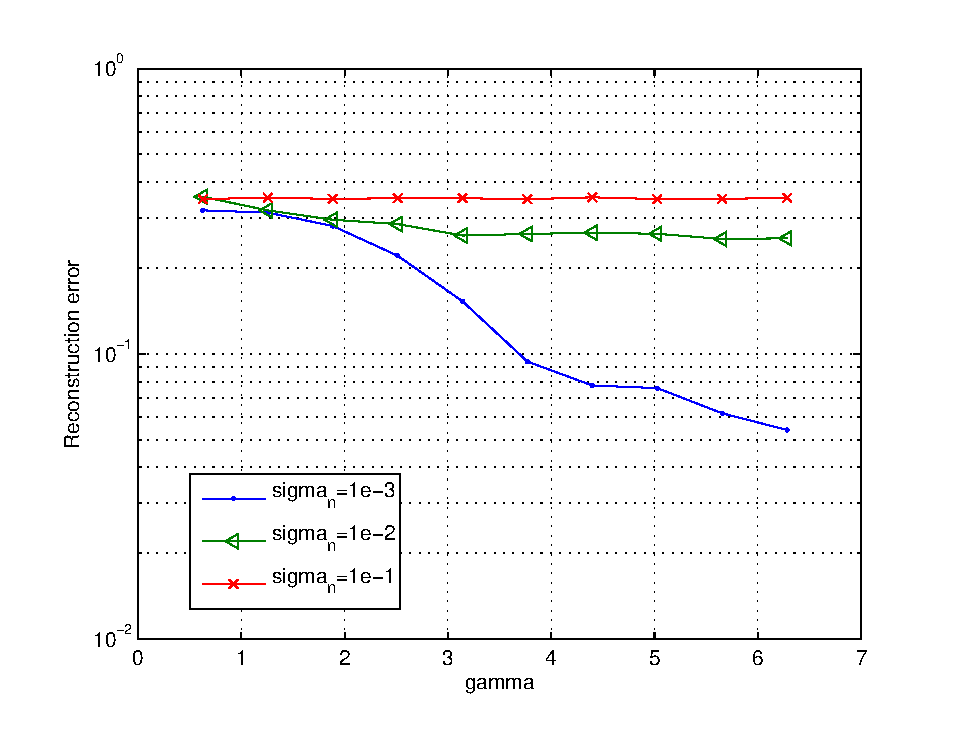
\includegraphics[width=7cm]{fig1a}
%   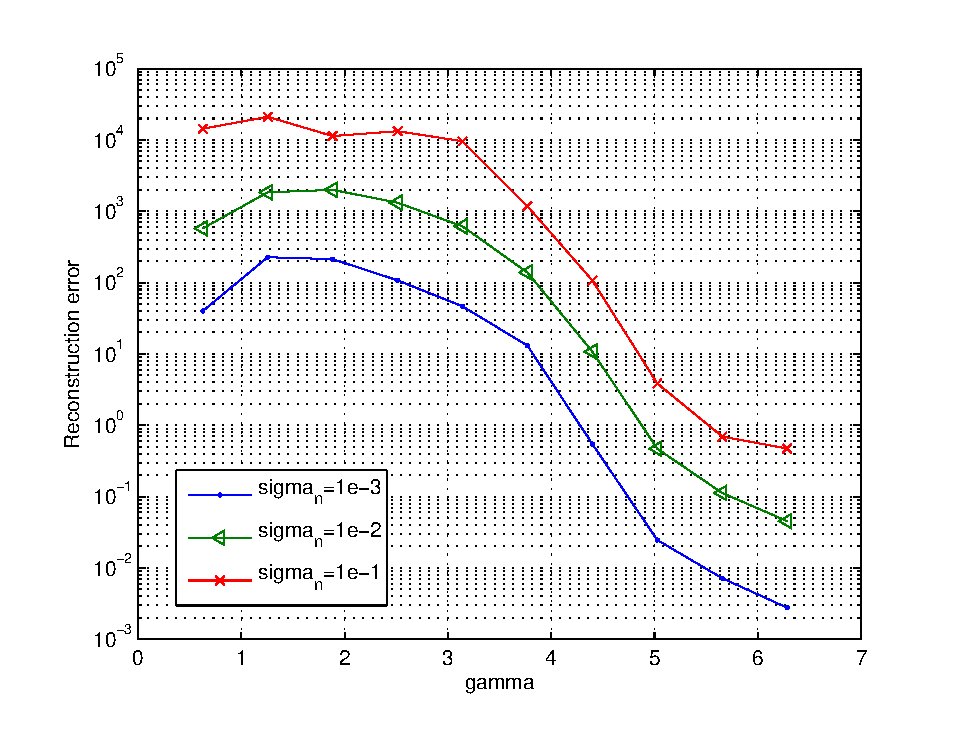
\includegraphics[width=7cm]{fig1b}
%   %\vspace{7.5cm}
%   \caption{Same experiment as in Figure \ref{fig:target_path}, with a limited angle of view
%     $\gamma=\pi$ (a), and $\gamma=1.4\pi$ (b).}
%   \label{fig:target_path_lim_aov}
% \end{figure}

% \begin{figure}[htp]
%   \centering
%   % \subfigure[]{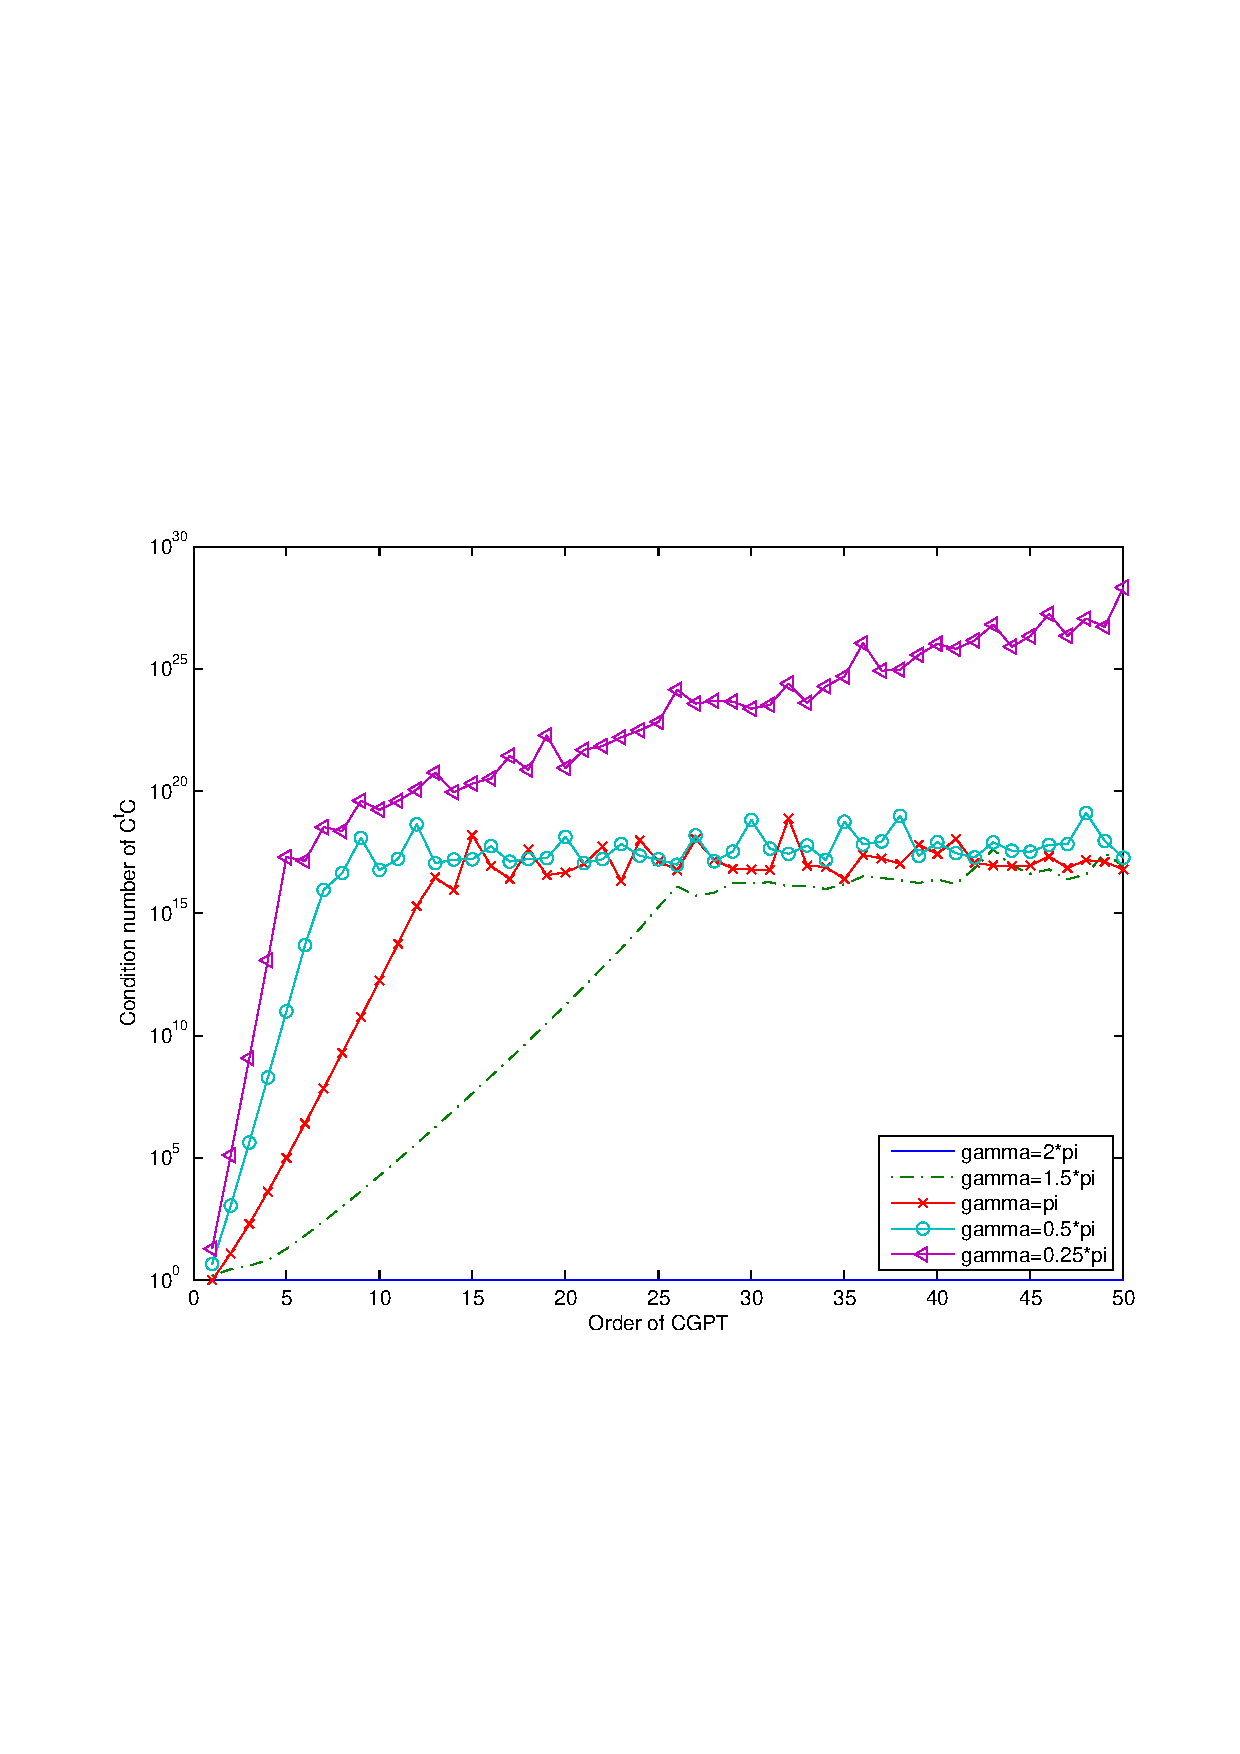
\includegraphics[width=6.5cm]{fig2a}}
%   % \subfigure[]{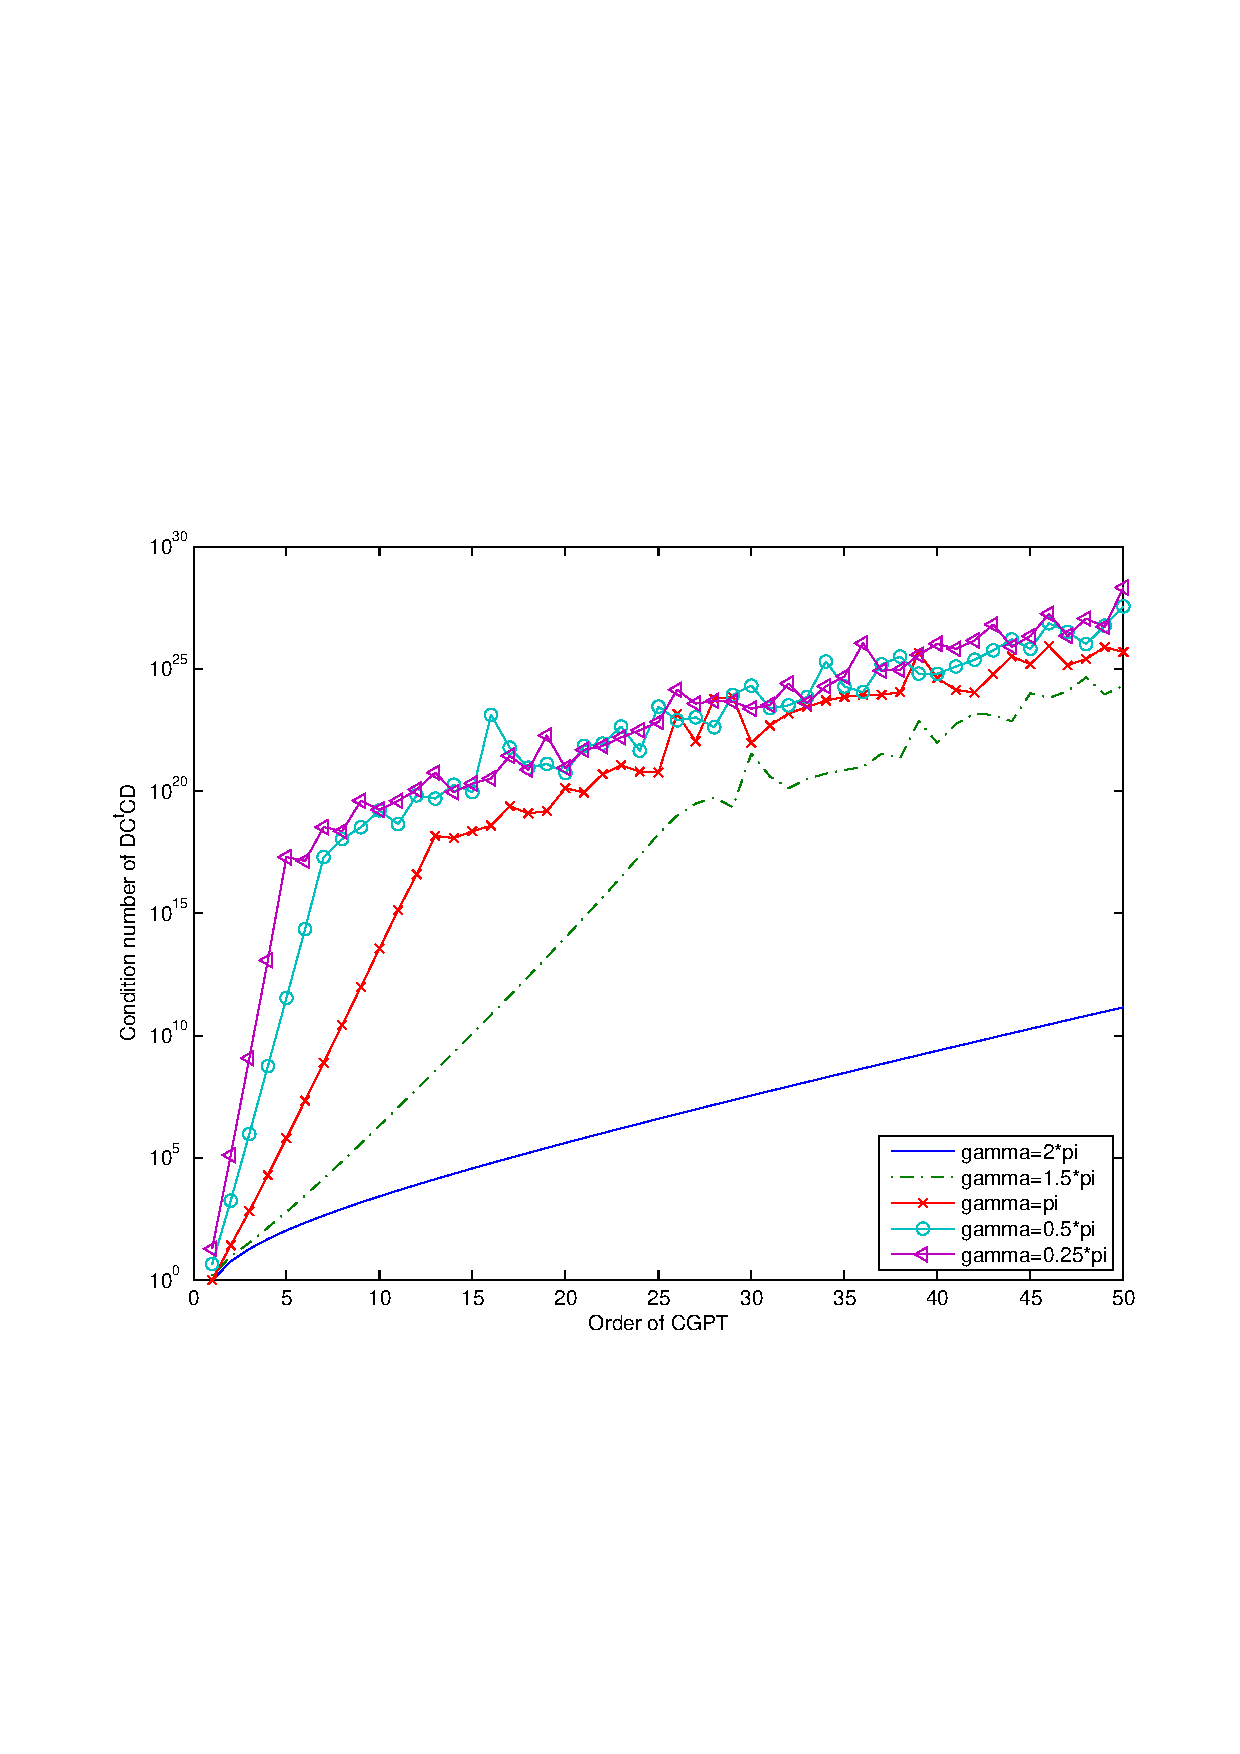
\includegraphics[width=6.5cm]{fig2b}}
%   % \subfigure[]{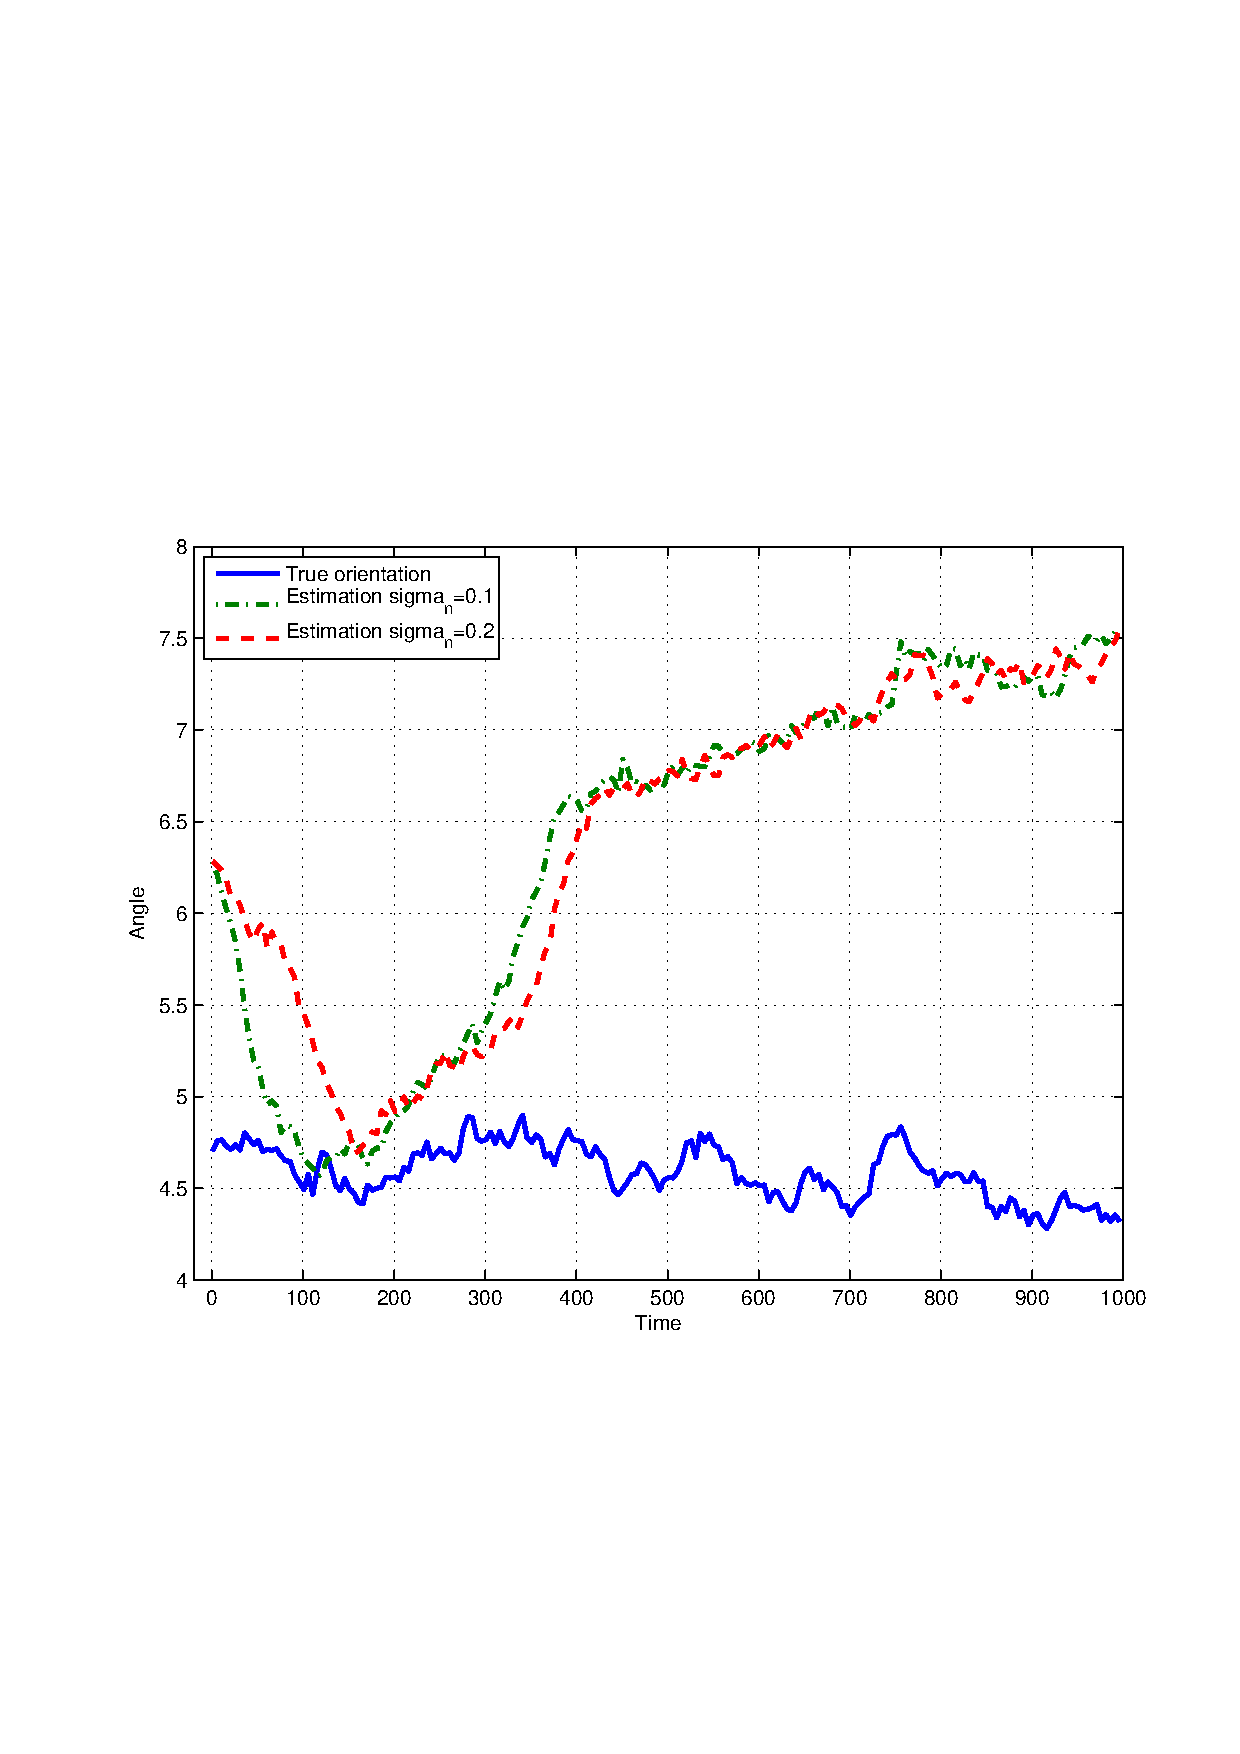
\includegraphics[width=6.5cm]{fig2c}}
%   \subfigure[]{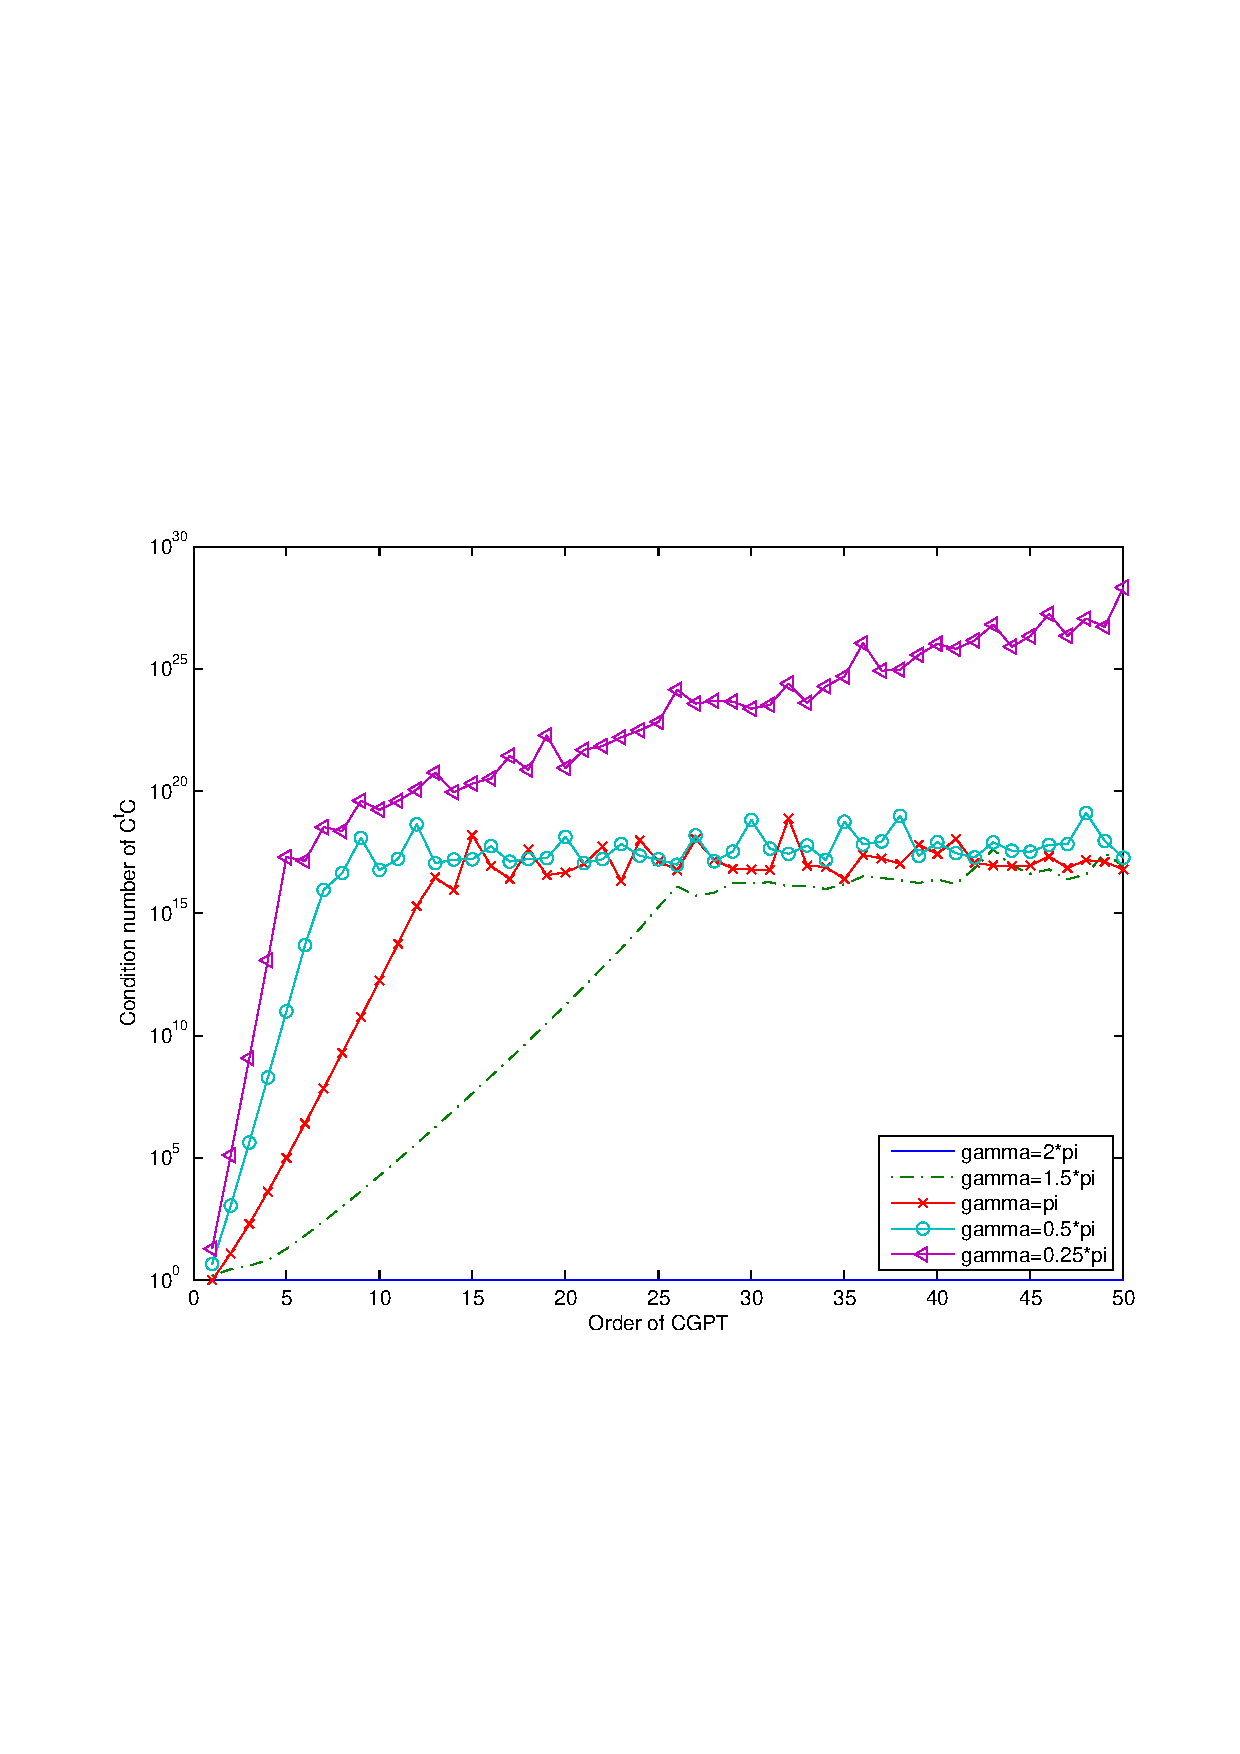
\includegraphics[width=6.5cm]{fig2a}}
%   \subfigure[]{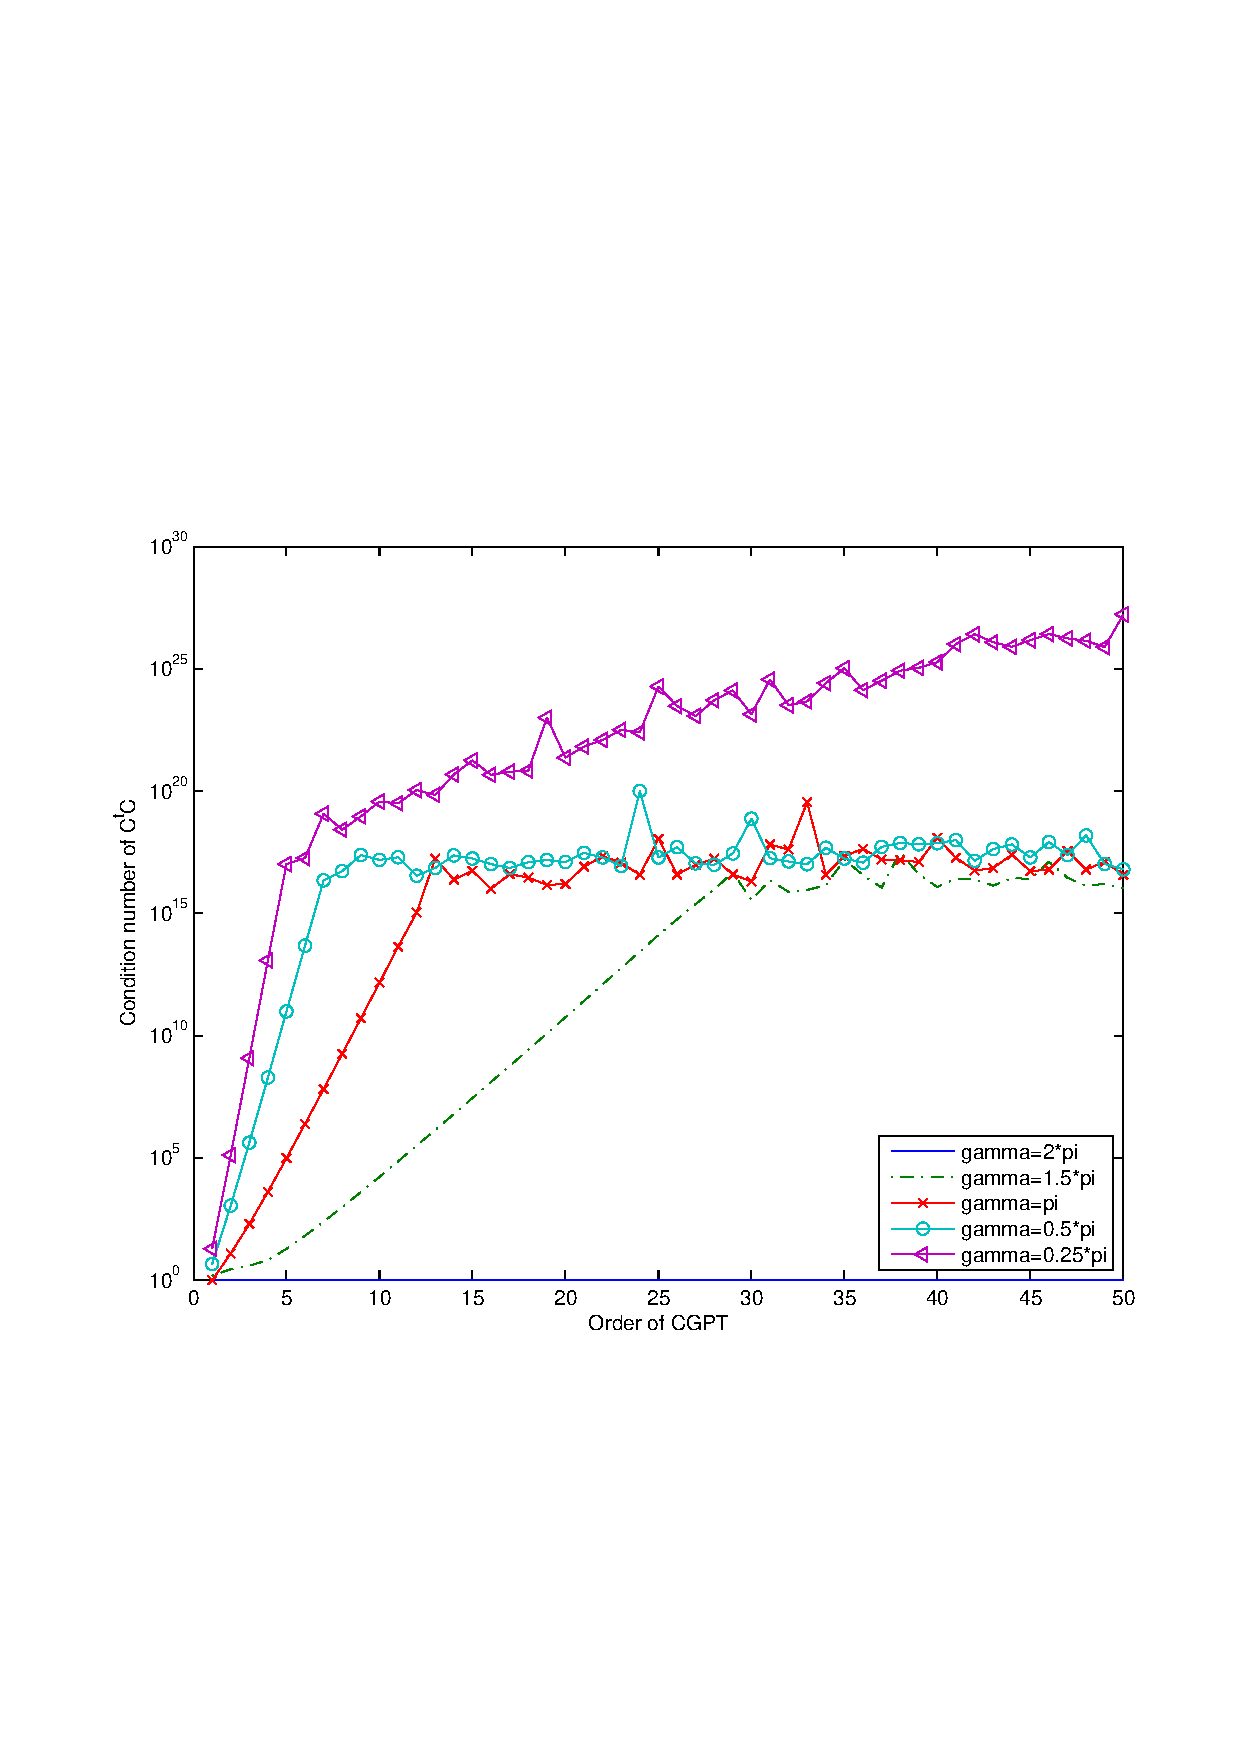
\includegraphics[width=6.5cm]{fig3a}}
%   \subfigure[]{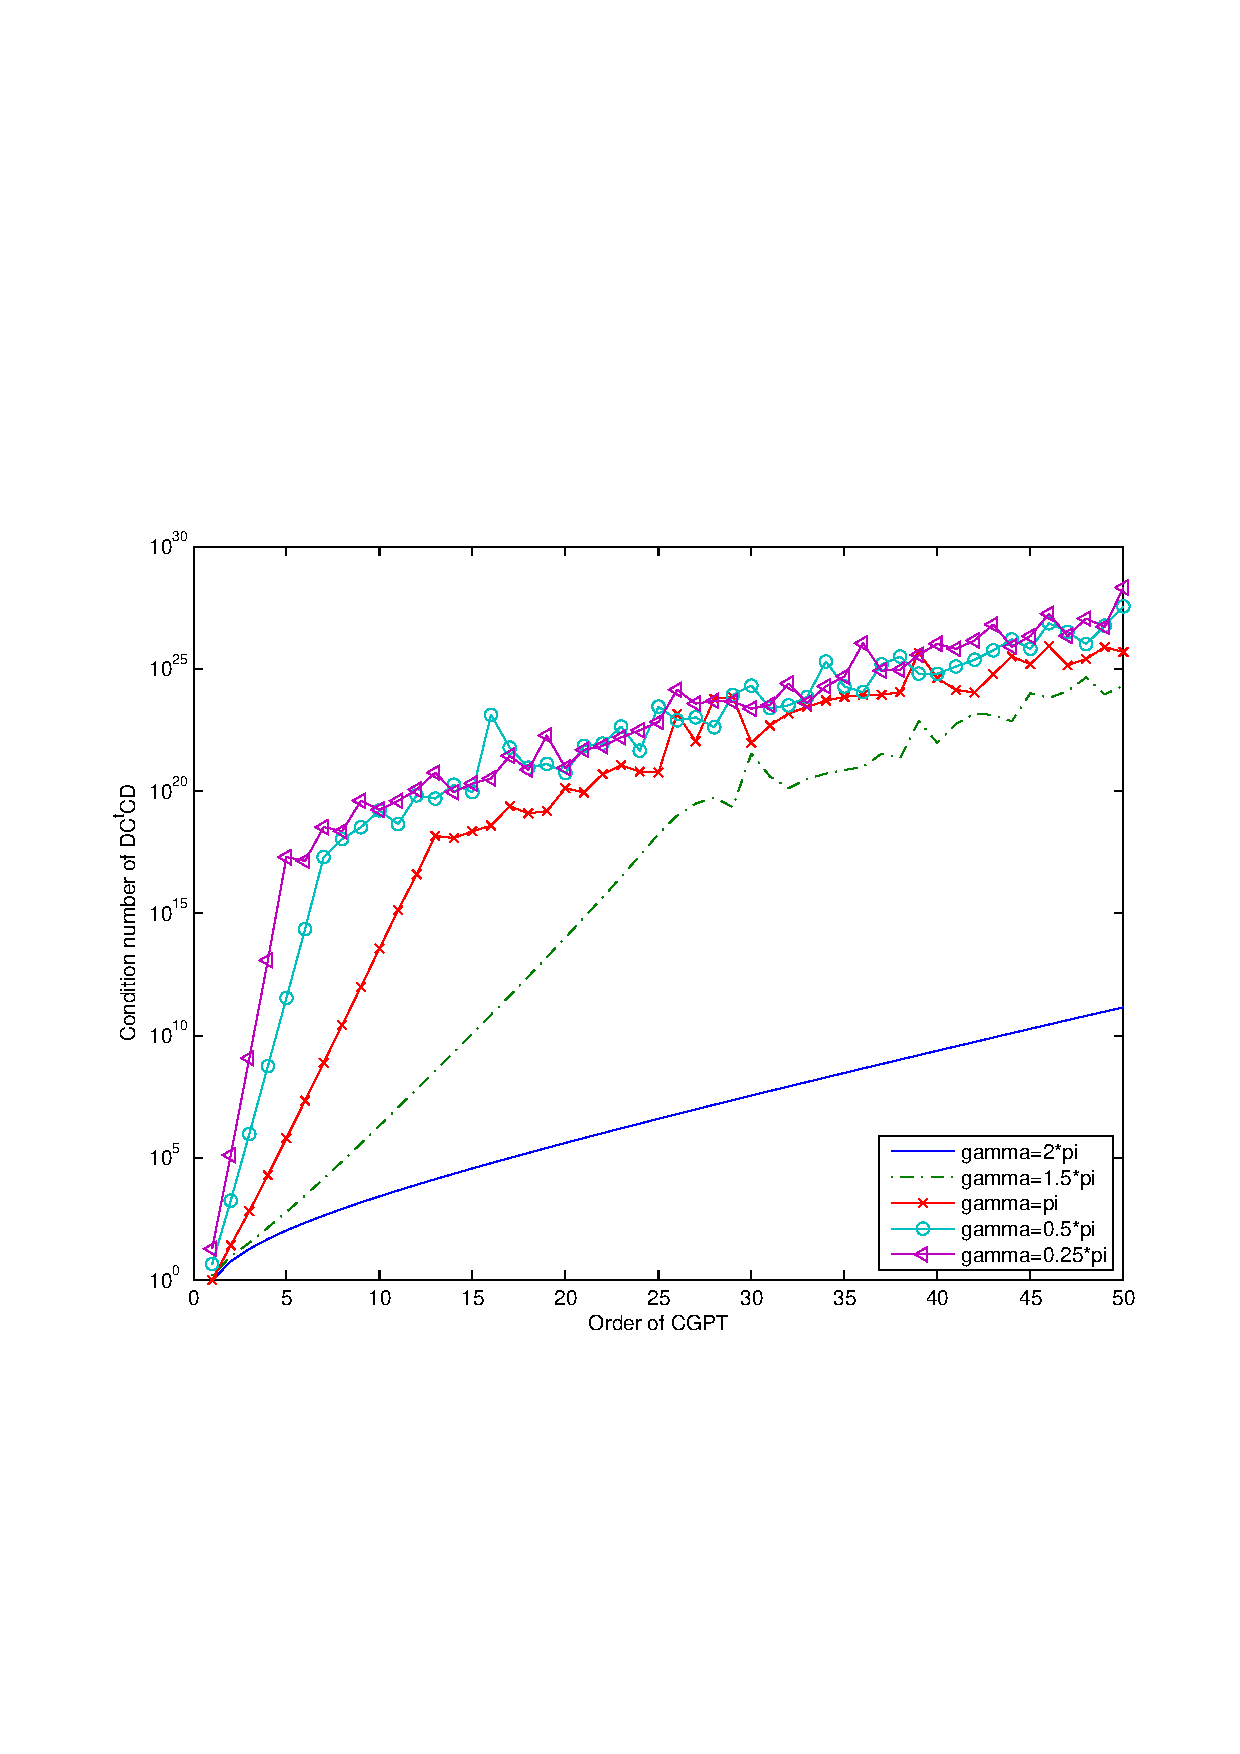
\includegraphics[width=6.5cm]{fig2b}}
%   \subfigure[]{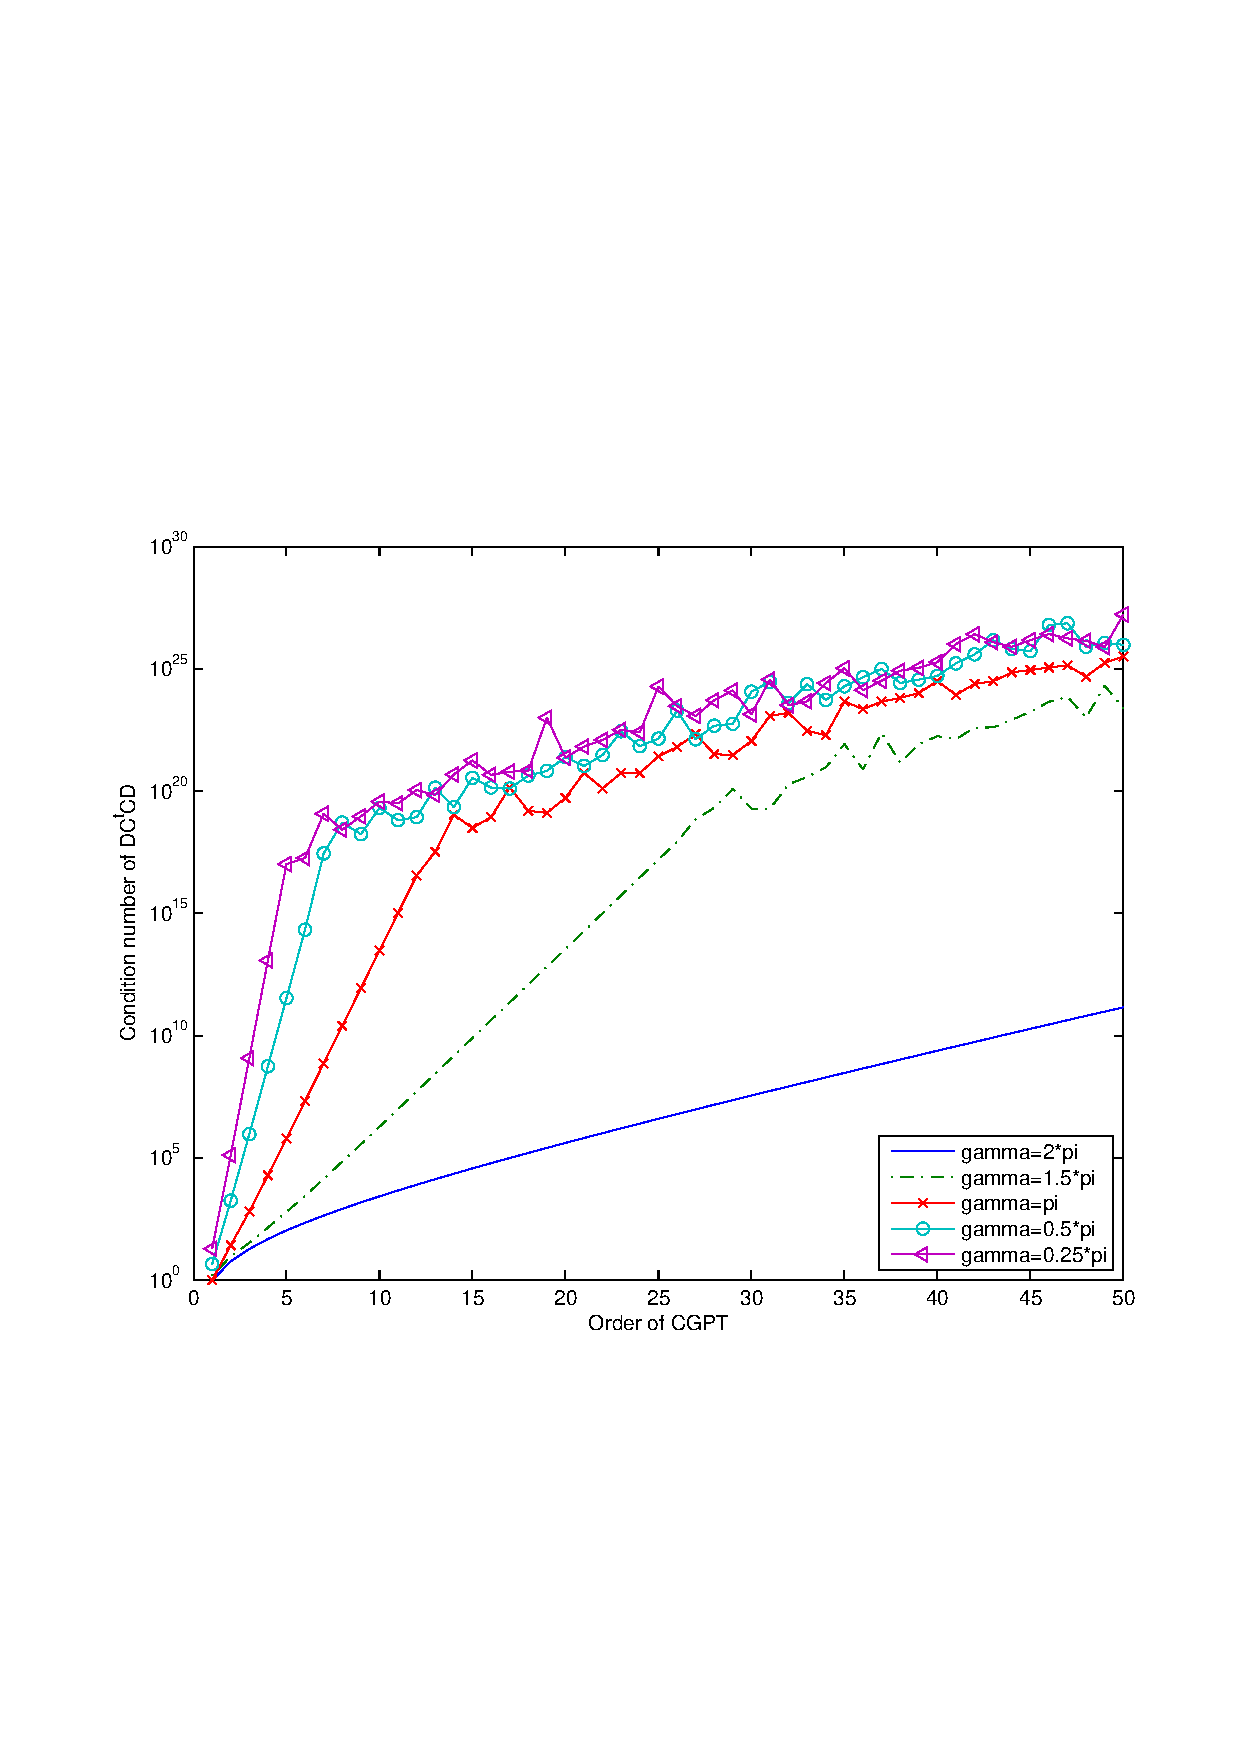
\includegraphics[width=6.5cm]{fig3b}}
%   \subfigure[]{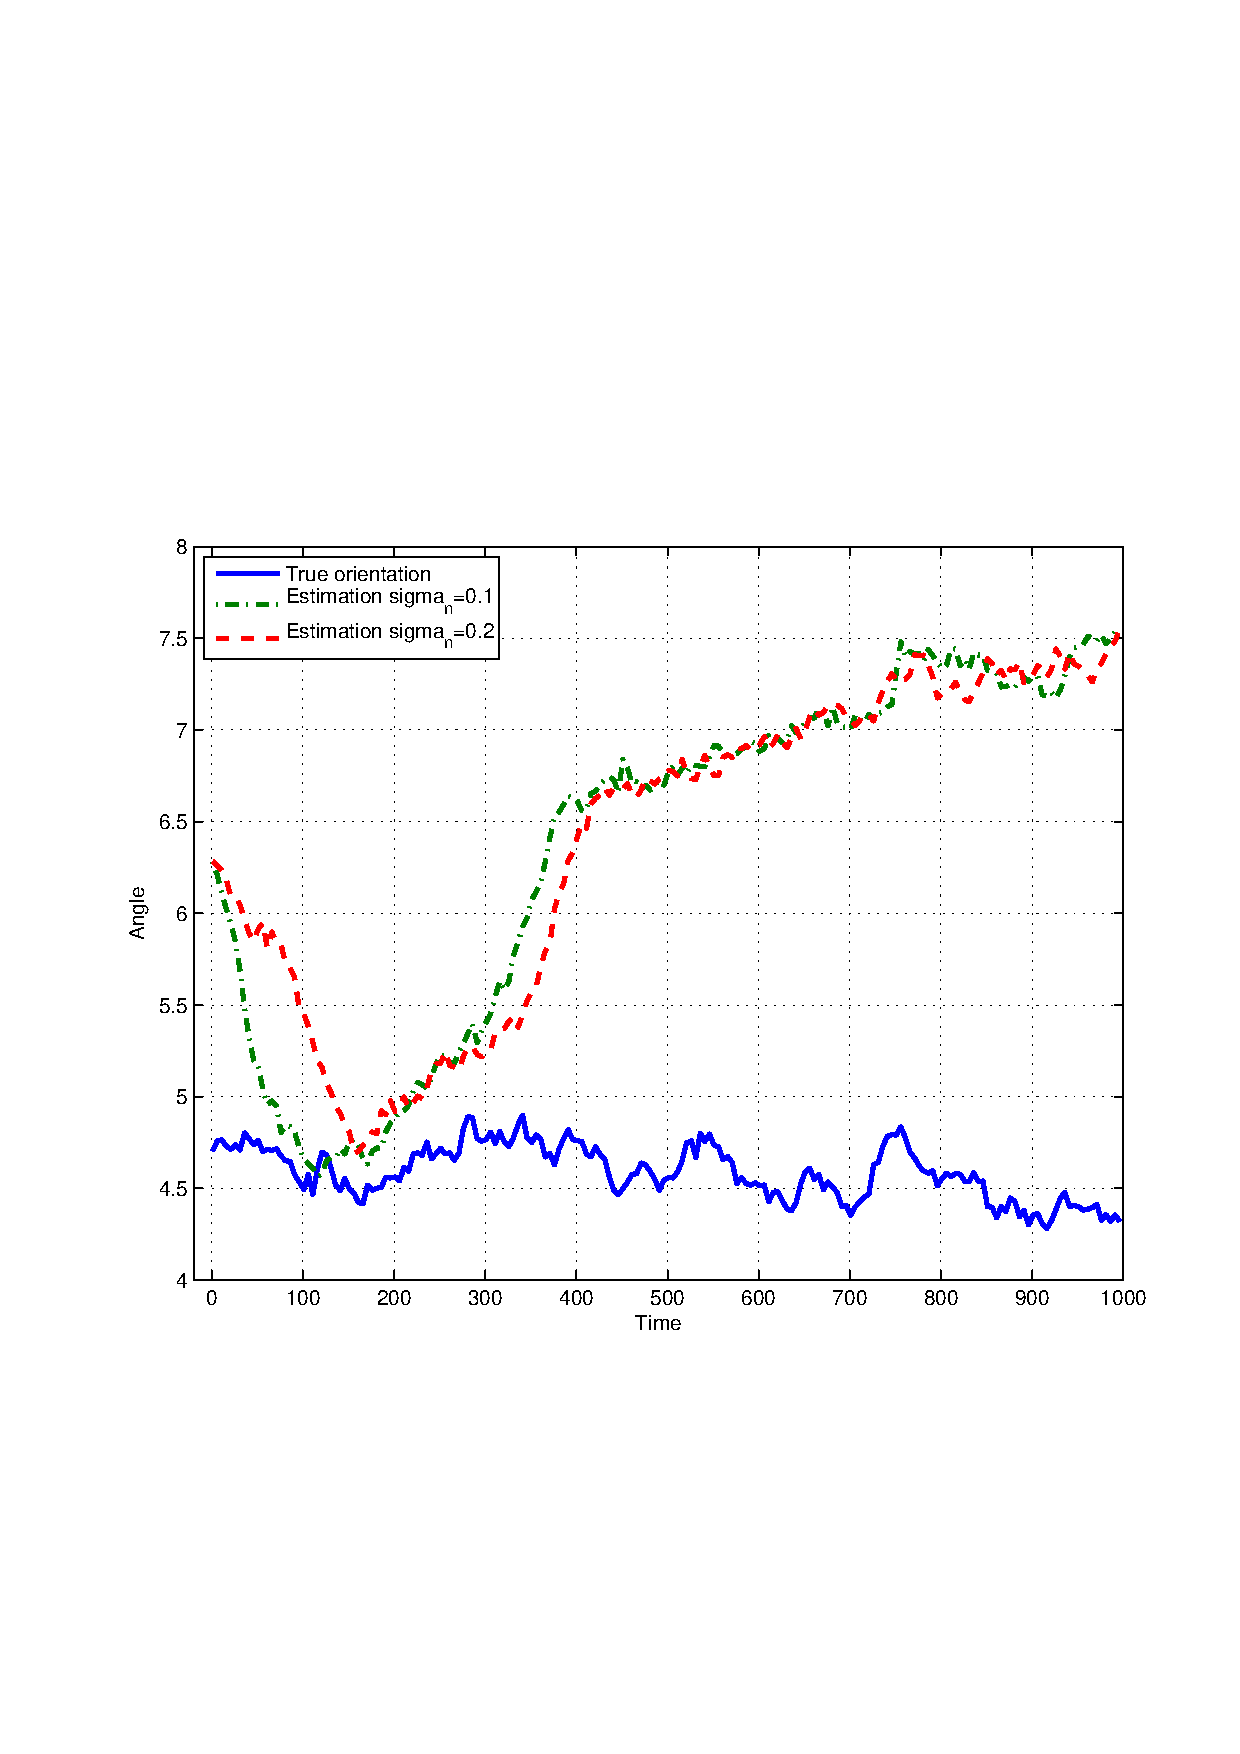
\includegraphics[width=6.5cm]{fig2c}}
%   \subfigure[]{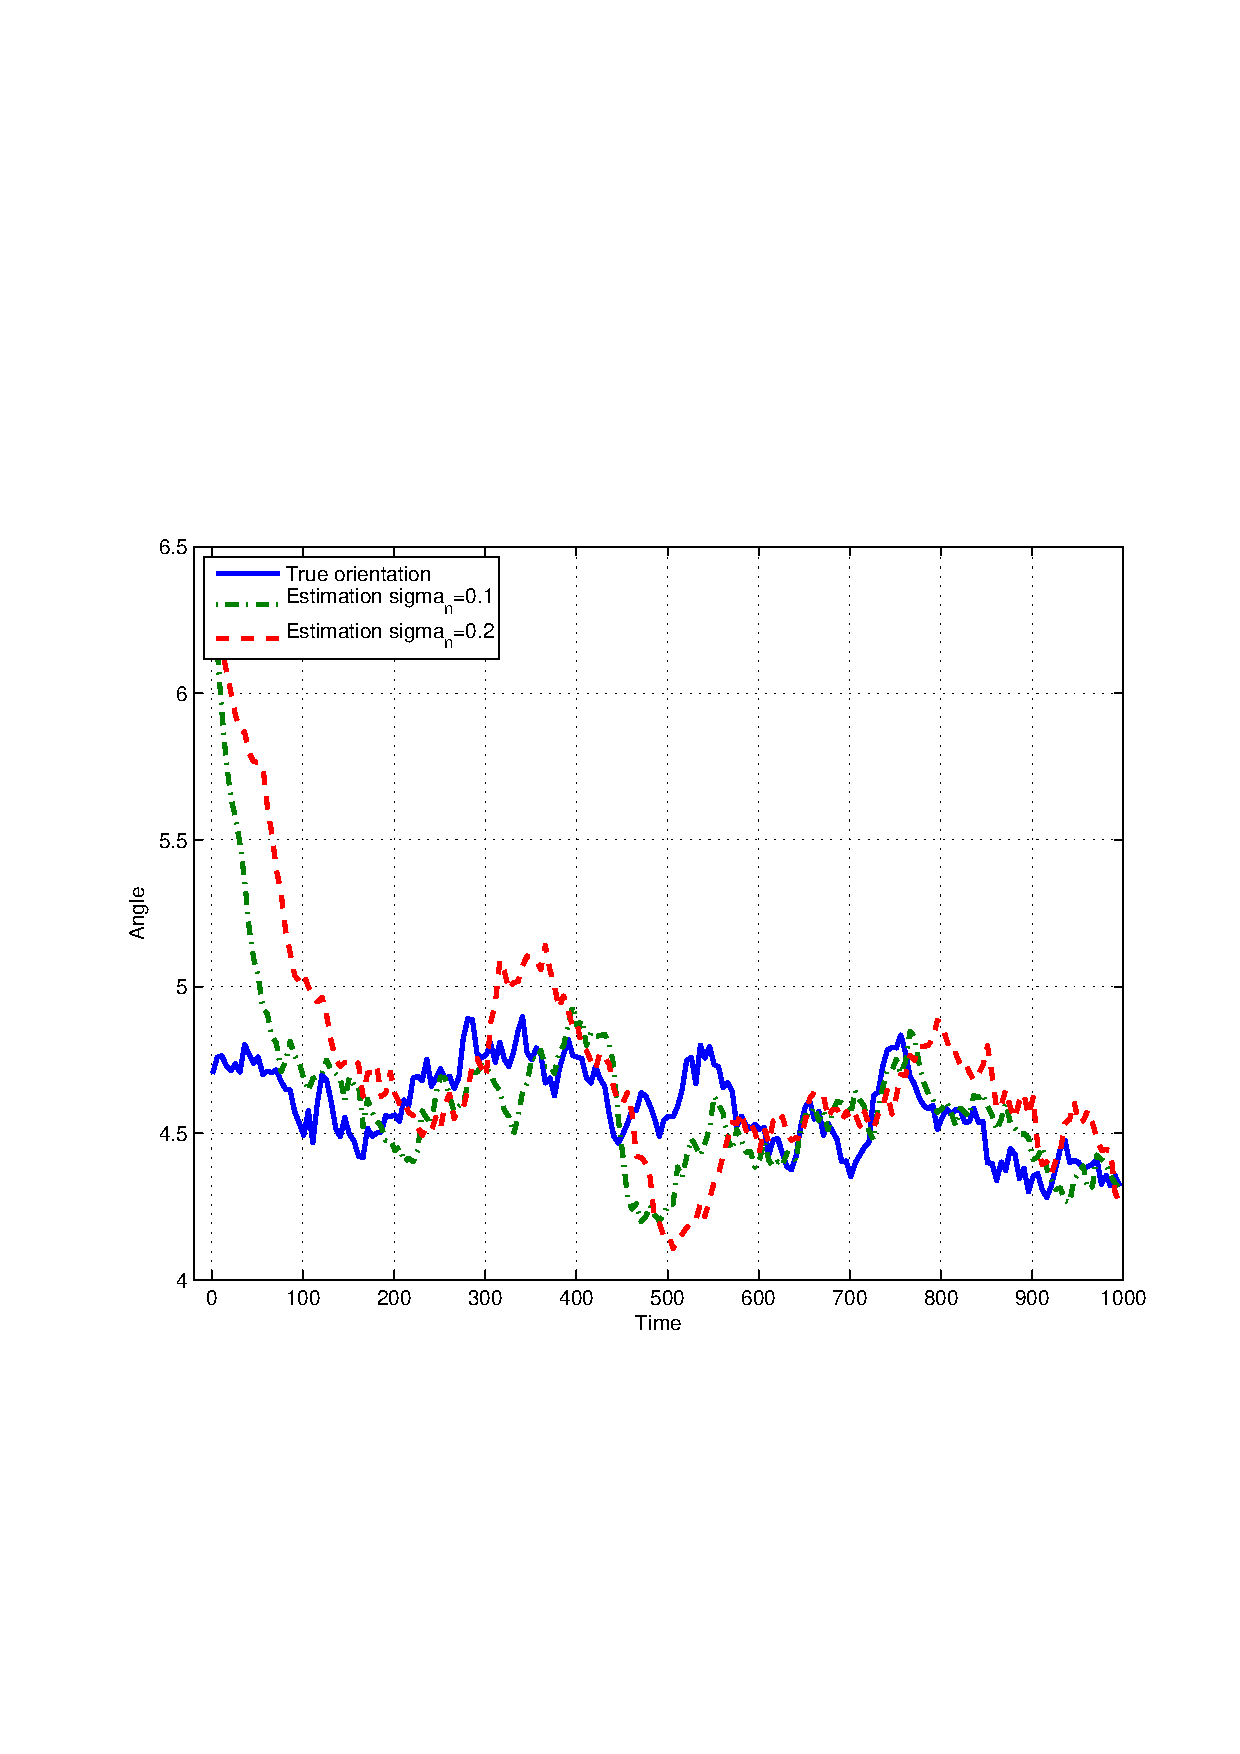
\includegraphics[width=6.5cm]{fig3c}}
%   \caption{Results of tracking using the configuration of Figure~\ref{fig:target_path_lim_aov} at
%     different noise levels. First row: coordinate in $x$-axis. Second row: coordinate in
%     $y$-axis. Last row: orientation. $\gamma=\pi$ and $\gamma=1.4\pi$ in the first and the second
%     column respectively.}
%   \label{fig:tracking_big_small_target}
% \end{figure}

%\graphicspath{{../figures/tracking_lim_aov/}}
\begin{figure}[htp]
  \centering
  \subfigure[]{\includegraphics[width=7cm]{tracking/lim_aov_1/tracking.eps}}
  \subfigure[]{\includegraphics[width=7cm]{tracking/lim_aov_2/tracking.eps}}
  \caption{Same experiment as in Figure \ref{fig:target_path}, with a limited angle of view
    $\gamma=\pi$. In Figure(a) sources/receivers are equally distributed between $[0,\gamma)$, while
    in Figure(b) they are divided into 5 groups.}
  \label{fig:target_path_lim_aov}
\end{figure}

\begin{figure}[htp]
  \centering
  \subfigure[]{\includegraphics[width=6.5cm]{tracking/lim_aov_1/pos_x.eps}}
  \subfigure[]{\includegraphics[width=6.5cm]{tracking/lim_aov_2/pos_x.eps}}
  \subfigure[]{\includegraphics[width=6.5cm]{tracking/lim_aov_1/pos_y.eps}}
  \subfigure[]{\includegraphics[width=6.5cm]{tracking/lim_aov_2/pos_y.eps}}
  \subfigure[]{\includegraphics[width=6.5cm]{tracking/lim_aov_1/orientation.eps}}
  \subfigure[]{\includegraphics[width=6.5cm]{tracking/lim_aov_2/orientation.eps}}
  \caption{Results of tracking using the configuration of Figure~\ref{fig:target_path_lim_aov} at
    different noise levels. First row: coordinate in $x$-axis. Second row: coordinate in
    $y$-axis. Last row: orientation. First and second column correspond to the configuration in
    Figure~\ref{fig:target_path_lim_aov} (a) and (b), respectively.}
  \label{fig:tracking_lim_aov_uni_nonuni}
\end{figure}




\section{Conclusion}
\label{sec:conclusion}

In this chapter we have provided a location and orientation tracking
of a mobile target from MSR measurements in the full- and
limited-view settings. In the limited-view case, the effect of noise is severe on
the tracking. However, if the arrays of receivers and transmitters
offer a good directional diversity, then satisfactory results can
be obtained. It would be interesting to generalize our algorithms
for tracking multiple targets. As a first step, a matching pursuit
algorithm \cite{mallat1999wavelet} would be appropriate for recognizing the
targets.
